\documentclass{ecnreport}

\stud{Option Robotique, EMARO-ARIA M1}
\topic{Computer Vision}

\begin{document}

\inserttitle{Computer Vision Lab}

\insertsubtitle{Labs 1-2: Calibration and pose computation}



\section{Content of this lab}

The goal is this lab is to perform camera calibration and pose computation. Do to so, we will use two C++ libraries:
\begin{itemize}
 \item OpenCV\footnote{Open source Computer Vision, http://opencv.org} to read images from files or camera, and perform low-level image processing
 \item ViSP\footnote{Visual Servoing Platform, http://visp.inria.fr} to manipulate 3D points, camera pose and use vectors and matrices.
\end{itemize}
The actual classes that are used are detailed in Appendix \ref{sec:classes}.

\subsection{The cameras}

Several IEEE-1394 Firewire cameras are available for this lab. Some of them have a low distortion while others are fish-eye cameras. We will consider the 
same framework to calibrate and perform pose computation for both, that is virtual visual servoing (VVS).

\subsection{Calibration landmarks}

Camera calibration and pose computation usually require to observe known objects. In our case we will consider a grid composed of 6$\times$6 points and
the OpenCV chessboard (see \Fig{fig:landmarks}).

\begin{figure}[h!]
 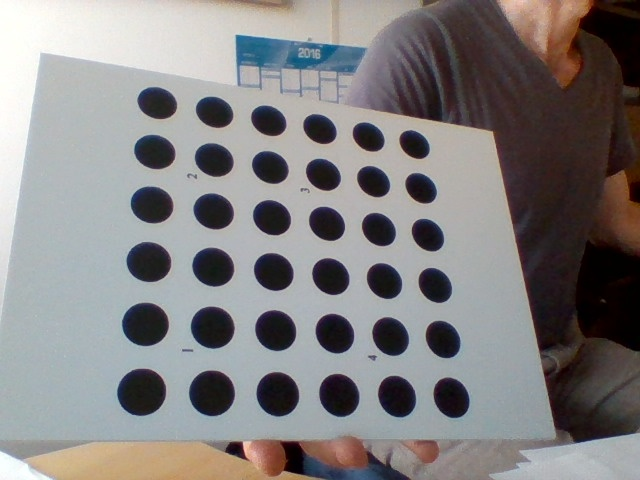
\includegraphics[width=.45\linewidth]{grid} ~~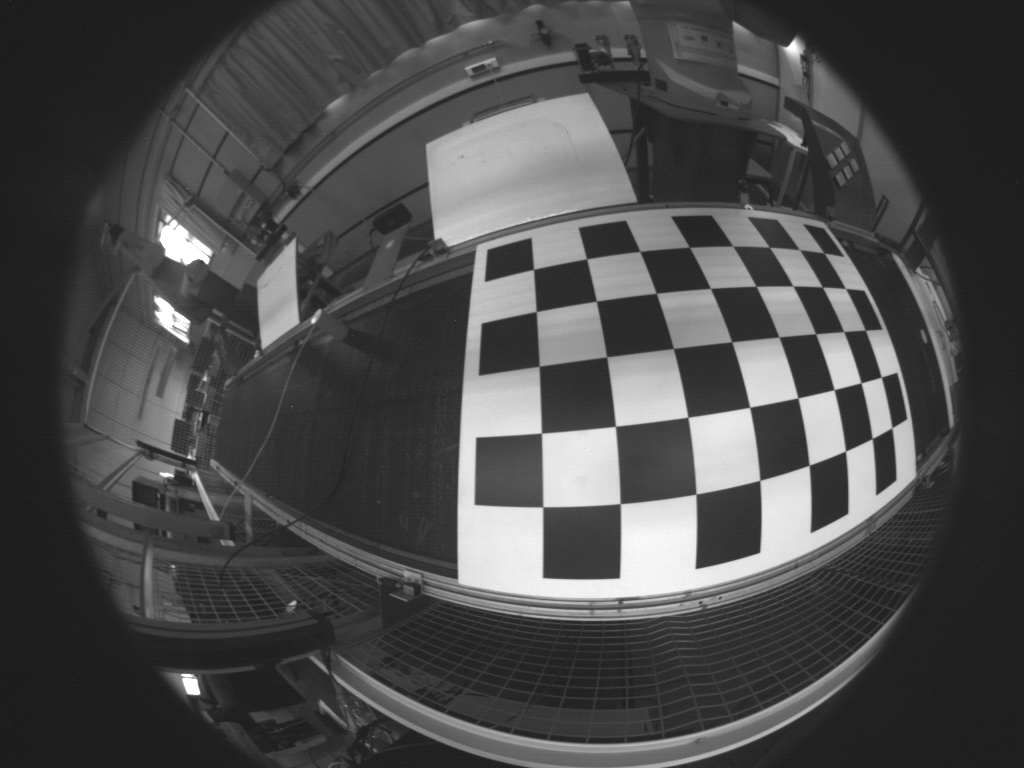
\includegraphics[width=.45\linewidth]{chessboard}
 \caption{Calibration landmarks, point grid with a low distortion camera (left) and OpenCV chessboard seen by a fish-eye camera (right).}
 \label{fig:landmarks}
\end{figure}

\newcommand{\xii}{{\boldsymbol{\xi}}}

In both cases, the interest points lie on a grid pattern of known dimension (rows, columns and inter-point distance). The 3D coordinates of those points
are thus known. The goal is to estimate the camera parameters $\xii$ and the camera poses $\M_i$ (one pose for each image) that minimize the reprojection error between the known 3D positions
and the extracted 2D (pixel) positions.

\subsection{Calibration procedure}

Calibration will begin by saving several images acquired from the camera. The calibration program will then have to read them and extract the interest
points. A virtual visual servoing scheme will then be used to minimize the error.
Assuming we are using $n$ images and that the calibration landmark is using $m$ points:
\begin{itemize}
 \item the reprojection error is of dimension $(2\times n\times m)$ (2 coordinates per point per image).
 \item the unknown is of dimension $(n_\xii + 6\times n)$ where $n_\xii$ is the number of parameters of the camera model.
\end{itemize}
The VVS is an optimization problem written as:
\begin{equation}\label{eq:calib}
 \xii, (\M_i)_i = \arg\min \norm{\s(\xii, (\M_i)_i) - \sd}^2
\end{equation}
where $\sd$ regroups the desired pixel coordinates of the interest points in each image and correspond to the extracted pixel positions, 
and where $\s(\xii, (\M_i)_i)$ is the pixel coordinates of the known 3D points when projected with intrinsic parameters $\xii$ and camera poses $(\M_i)_i$.


From an estimation of $\xii$ and $(\M_i)_i$, the 3D point $\X({}^o X,{}^o Y,{}^o Z)$ whom coordinates are expressed in the object frame $\Frame{o}$ can easily be projected in pixel coordinates.
The coordinates of $\X$ in the camera frame yield:
\begin{equation}\label{eq:framechange}
 \left[\begin{array}{c}{}^c\X\\1\end{array}\right]=   \left[\begin{array}{c}X\\Y\\Z\\1\end{array}\right] =\M_i\left[\begin{array}{c}\X\\1\end{array}\right]
\end{equation}

For a classical perspective camera model, we have $\xii = (p_x, p_y, u_0, v_0)$ and the perspective projection:
\begin{equation}\label{eq:projection}
 \left\{\begin{array}{ll}
  u &= p_x.X/Z + u_0 \\
  v &= p_y.Y/Z + v_0
 \end{array}\right.
\end{equation}

From \eqref{eq:framechange} and \eqref{eq:projection} the full projection function $\s(\xii, (\M_i)_i)$ can be defined.\\ 

\eqref{eq:calib} can then be resolved from an initial guess on $\xii$ and $(\M_i)_i$ with a simple gradient descent. 
The error derivative with regards to intrinsic parameters and camera poses has the following structure:
\newcommand{\der}{\text{d}}
\begin{equation}\label{eq:jacob}
 \der\s =  \left[\begin{array}{ccccc}
           \J_1 & \L_1 &  0 &  \hdots & 0 \\ 
           \J_i & 0 & \L_i &  \hdots & 0 \\
           \vdots& \vdots & \ddots & \ddots & \vdots\\
           \J_n & 0 & \hdots & 0 & \L_n
            \end{array}\right]
            \left[\begin{array}{c}\der\xii \\ \v_1 \\ \vdots \\ \v_n\end{array}\right]
             = \J\der\x
\end{equation}
where:
\begin{itemize}
\item $\J_i$ is the derivative of the reprojection of the points of image $i$ with regards to the intrinsic parameters (dimension $(2m)\times n_\xii$)
 \item $\L_i$ is the interaction matrix of the reprojection of the points of image $i$ (dimension $(2m)\times 6$)
 \item $\der\xii$ is the change in the intrinsic parameters (dimension $n_\xii$) 
 \item $\v_i$ is the velocity screw of the estimated camera pose of image $i$ (dimension $6$)
 \item As a consequence, $\J$ is of dimension $(2mn)\times (n_\xii+6n)$ and $\der\x$ is of dimension  $(n_\xii+6n)$
\end{itemize}
The gradient descent allows computing iteratively new values for $\xii$ and $(\M_i)_i$ with:
\begin{equation}
 \der\x = \left[\begin{array}{c}\der\xii \\ \v_1 \\ \vdots \\ \v_n\end{array}\right] = -\lambda\Jp(\s - \sd)
\end{equation}
$\xii$ can then be updated simply with $\xii^{\text{new}} = \xii + \der\xii$.\\
$\M_i$ is updated with $\v_i$ through the exponential map: $\M_i^{\text{new}} = \exp(-\v_i)\times\M_i$.\\

Matrices $\J_i$ and $\L_i$ are of course not constant and depend on the several considered points. 

\subsection{Pose computation procedure}

In pose computation we assume the camera is already calibrated and we are dealing from the image stream of the camera.
We are just looking for the current pose $\M$ of the camera.
The minimization problem is thus the same as \eqref{eq:calib} but is highly simplified:
\begin{equation}\label{eq:pose comp}
\M = \arg\min \norm{\s(\M) - \sd}^2
\end{equation}The exact same algorithm as for the calibration can thus be used, without having to consider intrinsic parameters or several images.
\eqref{eq:jacob} is thus simplified to :
\begin{equation}
 \der\s =  \L\v
\end{equation}
The initial guess for $\M$ still has to be done, but when a new image comes the guess is of course the previous estimation of $\M$ as we assume the image stream 
correspond to very close poses of the camera.


\section{Calibration implementation}


\subsection{Expected work}

During the lab the files will be modified and others will be created.
At the end of the lab, please send by email a zip file allowing to compile and test the program.

You may answer the questions by inserting comments in the code at the corresponding lines.



\newpage

\section{Building the \texttt{Robot} class}

\subsection{Incomplete methods}


\begin{itemize}
\medskip\item[\textbf{\underline{Q1}}]  Compile and execute the program. According to the \texttt{main.cpp} file, the robot is following some velocity setpoints defined in the $(x,y,\theta)$ space. In which files are the following elements defined:
\begin{enumerate}
\item \texttt{DefaultEnvironment}
\item \texttt{DefaultCartesianSetpoint}
\item \texttt{Environment}
\end{enumerate}

\medskip\item[\textbf{\underline{Q2}}] Explain the signature of   \texttt{DefaultCartesianSetpoint}, especially the way to pass arguments. 
From the \texttt{main()} function, can \texttt{i} be modified in \texttt{DefaultCartesianSetpoint}? What about \texttt{vx}?

\medskip\item[\textbf{\underline{Q3}}] In practice it is often impossible to control a ground robot by sending $(x,y,\theta)$ velocities. A classical way to control such a robot is to send a setpoint with a linear velocity $v$ and an angular velocity $\omega$, expressed in the robot frame as shown in \Fig{fig:dd}.



The corresponding model is quite simple:
\begin{equation}
\left\{\begin{array}{ll}
\dot x &= v\cos \theta \\
\dot y &= v\sin \theta \\
\dot \theta &= \omega
\end{array}\right.
\end{equation}

Implement such a function in \texttt{Robot::MoveVW}. This method should compute the $(x,y,\theta)$ velocities from $(v,\omega)$ and then call the \texttt{Robot::MoveXYT} method. 

\medskip\item[\textbf{\underline{Q4}}] Now that a realistic way to control the robot is possible, should the \texttt{Robot::MoveXYT} method stay available for external use? What can we do in the \texttt{robot.h} file to make it impossible to use it from outside the \texttt{Robot} class?

\medskip\item[\textbf{\underline{Q5}}] When a robot is equipped with two actuated wheels, a simple model is the differential drive model, as shown in \Fig{fig:dd}. Assuming the two wheels have a radius $r$ and are separated with a distance $b$, then the kinematic model yields:
\begin{equation}\label{eq:dk}
\left\{\begin{array}{ll}
v &= \displaystyle r \frac{\omega_l + \omega_r}{2} \\
\omega &= \displaystyle r \frac{\omega_l - \omega_r}{2b}
\end{array}\right.
\end{equation}As in question 3, implement such a function in the \texttt{Robot::RotateWheels} method, so that it can be possible to control the robot by sending wheel velocities. You may want to define new attributes in the \texttt{Robot} class in order to initialize the radius and base distance through the \texttt{Robot::InitWheel} method. We use the following values:
\begin{equation}
\left\{\begin{array}{ll}
r &= 0.05 m \\
b &= 0.3 m
\end{array}\right.
\end{equation}
The method should rely on \texttt{Robot::MoveXYT} after having computed the $(x,y,\theta)$ velocities from $(\omega_l, \omega_r)$.

\medskip\item[\textbf{\underline{Q6}}] By using the \texttt{wheels\_init\_} attribute, make sure that it is impossible to do anything in \texttt{Robot::RotateWheels} if the radius and base have not been initialized.


\subsection{Velocity limits}

With the current simulation, we can control the robot:
\begin{itemize}
\item by sending linear and angular velocity setpoint with \texttt{Robot::MoveVW}
\item or by sending wheel velocities with \texttt{Robot::RotateWheels}
\end{itemize}

These two methods call \texttt{Robot::MoveXYT}\footnote{which should not be calable anymore from outside the \texttt{Robot} class} and the robot can reach any velocity. In practice, the wheels have a limited velocity at $\pm$80 round per minute (rpm).

\medskip\item[\textbf{\underline{Q1}}] Modify the \texttt{Robot::InitWheels} method in order to pass a new argument that defines the wheel angular velocity limit. You may need to define a new attribute of the \texttt{Robot} class to store this limit. Update the \texttt{main.cpp} file with the value in radian per second corresponding to 80 rpm.

\medskip\item[\textbf{\underline{Q2}}] Modify the \texttt{Robot::RotateWheels} method in order to ensure that the applied velocities $(\omega_l, \omega_r)$ are within the bounds.
The method should also print a message if the velocity setpoint is too high.
Note that if you just saturate the velocities, the robot motion will be different. A scaling is a better strategy, in this case we keep the same ratio between $\omega_l$ and $\omega_r$.

\medskip\item[\textbf{\underline{Q3}}] Although the robot actually moves by having its wheels rotate, it would be easier to be able to send linear and angular velocity setpoints. Modify the 
\texttt{Robot::MoveVW} method so that a $(v,\omega)$ setpoint is changed to a $(\omega_l,\omega_r)$ setpoint that will then be called through \texttt{Robot::RotateWheels}. Apply the default $(v,\omega)$ trajectory in the simulator. The inverse of model \eqref{eq:dk} yields:
\begin{equation}
\left\{\begin{array}{ll}
\omega_l &= \displaystyle \frac{v + b\omega}{r} \\
\omega_r &= \displaystyle \frac{v - b\omega}{r}
\end{array}\right.
\end{equation} 

\end{itemize}


\section{Sensors}

The \texttt{sensor.h} files defines a \texttt{Sensor} class that has four methods:
\begin{itemize}
\item \texttt{void Init}: initializes the relative pose between the sensor and the robot
\item \texttt{virtual void Update}: updates the measurement from the robot current position
\item \texttt{void Print}: prints the current measurement
\item \texttt{void Plot}: plots the measurement history       
\end{itemize}
The \texttt{Update} method is defined as a pure virtual function, which makes the \texttt{Sensor} class a abstract class. It is thus impossible to declare a variable to be of \texttt{Sensor} type, as this class is only designed to build daughter-classes depending on the sensor type.

The \texttt{Robot} class already has a attribute called \texttt{sensors\_} which is a vector of \texttt{Sensor*}. As the \texttt{Sensor} class is abtract it is forbidden to use it by itself, but pointers are still possible.


\subsection{Range sensors}


\begin{itemize}
\medskip\item[\textbf{\underline{Q1}}] Create a \texttt{sensor\_range.h} file that defines a \texttt{SensorRange} class that is derived from \texttt{Sensor}. The \texttt{Update} method has to be defined so that the code compiles. For now, just make the method print something to the screen.

\medskip\item[\textbf{\underline{Q2}}] Include this file in \texttt{main.cpp} and declare a \texttt{SensorRange} variable.  We will use a front range sensor placed at $(0.1, 0,0)$ in the robot frame. Call the \texttt{Update} method at the beginning of the \texttt{for} loop. Run the program and ensure that the sensor is updated.

\medskip\item[\textbf{\underline{Q3}}] In this question we will build the \texttt{Update} function. This sensor should return the distance to the first wall in its x-axis. The sensor can thus be simulated in two steps:
\begin{enumerate}
\item Compute the absolute position and orientation of the sensor. As the robot is passed to the \texttt{Update} method, we can use its own $(x_r,y_r,\theta_r)$ position and the relative position $(x_s,y_s,\theta_s)$ of the sensor to get the absolute sensor position:
\begin{equation}
\left\{\begin{array}{ll}
x &= x_r + x_s\cos\theta_r - y_s\sin\theta_r \\
y &= y_r + x_s\sin\theta_r + y_s\cos\theta_r \\
\theta &= \theta_r + \theta_s
\end{array}\right.
\end{equation}
\item Compute the distance to the nearest wall. In the environment variable, the walls are defined by a list of points available in \texttt{envir.walls}. \Fig{fig:dist} shows a configuration where the sensor is at $(x,y,\theta)$ and is facing a wall defined by $(x_1,y_1)$ and $(x_2,y_2)$.

In this case, the distance to the wall is:
\begin{equation}
d = \frac{x_{1} y_{2} - x_{1} y - x_{2} y_{1} + x_{2} y + x y_{1} - x y_{2}}{x_{1} \sin\theta - x_{2} \sin\theta - y_{1} \cos\theta + y_{2} \cos\theta}
\end{equation}
The computed distance is positive if the wall is in front of the sensor, and negative if it is behind (in this case this wall is actually not measured). Also, the denominator may be null if the wall is parallel to the sensor orientation.
\end{enumerate}
Define the \texttt{Update} function so that it updates the attribute \texttt{s} of the sensor with the distance to the nearest wall. 

\medskip\item[\textbf{\underline{Q4}}] At the end of the \texttt{Update} method, add the command to append the measurement history: \\\texttt{s\_history\_.push\_back(s\_);}\\
At the end of the program call the \texttt{Plot} method of the range sensor in order to display the measurements.
\end{itemize}

\appendix

\section{Main classes}\label{sec:classes}

\end{document}
